\documentclass[11pt, leqno]{article}
\usepackage[utf8]{inputenc}
\usepackage{polski}
\usepackage{a4wide}

\usepackage{graphicx}
\usepackage{amsmath}
%\usepackage{bbm}
\usepackage{amsthm}
\usepackage{amssymb}
\usepackage{algorithmic}
\usepackage{ulsy}
\usepackage[usenames,dvipsnames]{color}
\usepackage{hyperref}
\hypersetup
{
    colorlinks=true,       	% false: boxed links; true: colored links
    linkcolor = OliveGreen,	% color of internal links
	 urlcolor = OliveGreen  	% color of external links
}
\newenvironment{Itemize}
{\begin{itemize}
  \setlength{\itemsep}{1pt}
  \setlength{\parskip}{0pt}
  \setlength{\parsep}{0pt}}
{\end{itemize}}
\renewcommand{\i}[1]{\textit{#1}}


\title{Inverse Kinematics for Binary Trees}
\date{\today}
\author{Marcin Januszkiewicz, Jakub Kowalski}


\begin{document}

\maketitle
\vspace{17em}
\tableofcontents
\newpage

\section{Sformułowanie zadania}
Zagadnienie kinematyki odwrotnej (\textit{ang.}\ inverse kinematics) dotyczy reprezentacji kończyn (ogólnie tzw.\ efektora) za pomocą geometrycznego modelu w którym kości estymowane są przez linie, natomiast stawom odpowiadają kąty. Zadaniem kinematyki odwrotnej jest znalezienie takich położeń stawów, dla których osiągana jest pożądana pozycja kończyny, np.~zamocowana w pewnym punkcie startowym dosięga ona zadanego punktu końcowego. Możliwe położenia stawów określone są przez minimalny i maksymalny kąt rozwarcia. Chromosom jest to lista kątów odpowiadających rozwarciom kolejnych stawów kończyny.

Rozpatrywana przez nas rozszerzona wersja standardowego zagadnienia dotyczy ,,kończyn'' o strukturze pełnego drzewa binarnego. Zadanie polega na znalezieniu ustawienia drzewa, w którym każdy punkt końcowy dotyka określonego punktu docelowego (punktów docelowych jest tyle samo co liści drzewa), a krawędzie drzewa nie stykają się z żadną znajdującą się na planszy przeszkodą.


\subsection{Format pliku wejściowego}
Scenariusz (plik zawierający informację o planszy oraz właściwościach drzewa) jest plikiem tekstowym o~następującej konstrukcji (linie rozpoczynające się od \# traktowane są jako komentarz):
\begin{verbatim}
# Wielkość planszy w poziomie
8
# Wielkość planszy w pionie
6
# Punkt startowy (wszystkie punkty podane są w notacji X Y)
3 5
# Punkty docelowe
1 1
5 1
6 1
7 5
# Specyfikacja drzewa
# Początkowy ciąg znaków (R|L)+ koduje umiejscowienie danej krawędzi w drzewie
# Każda krawędź opisana jest za pomocą długości oraz minimalnej
# i maksymalnej miary kąta stawu względem krawędzi poprzedzającej
L 4 0 360
LL 2 0 360
LR 2 0 360
R 3 0 360
RL 4 0 360
RR 1 0 360
# Znajdujące się na planszy przeszkody definiowane są jako linie.
# Linia pomiędzy punktami (x1, y1) a (x2, y2) podawana jest w formacie 
# x1 y1 x2 y2
1 2 2 2
2 2 2 4
2 4 1 4
1 4 1 2
4 2 5 2
5 2 5 4
5 4 4 4
4 4 4 2
7 2 8 2
8 4 7 4
7 4 7 2
\end{verbatim}

Przypisanie punktów docelowych do liści drzewa odpowiada trawersowaniu go od lewej do prawej, tak więc pierwszy punkt docelowy zostanie przypisany do krawędzi \texttt{LL}, drugi do \texttt{LR}, trzeci do \texttt{RL} itd.

\section{Obsługa programu}
Graficzny interfejs użytkownika, wykorzystywany przez program testowy, przedstawiony jest na rysunku \ref{fig:gui}.
\begin{figure}[h!]
	\centering
	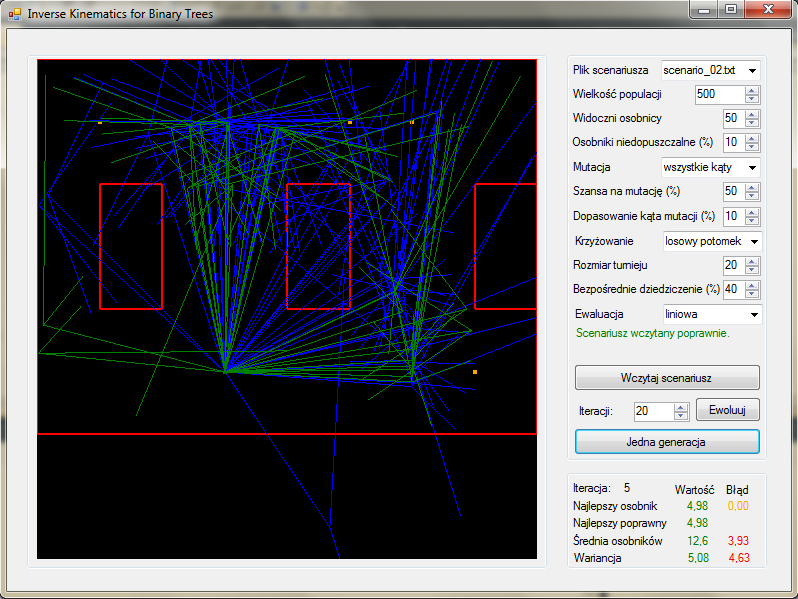
\includegraphics[scale=0.5]{gui}
	\caption{Interfejs programu}
	\label{fig:gui}
\end{figure}

Program pozwala wybrać jeden z przygotowanych plików scenariusza oraz określić podstawowe parametry ewolucji a także wybrać kombinację stosowanych przy ewolucji operatorów. Po wczytaniu scenariusza można uruchomić ewolucję od razu na kilka pokoleń zgodnie z~przekazanymi danymi lub sprawdzać jej zachowanie krok po kroku.

Statystyki aktualnej populacji pozwalają ocenić osobników (pokazywane są wartości błędu i minimalizowanej funkcji celu dla osobnika najlepszego w całej populacji, najlepszego bezbłędnego oraz wartości średnie), a także ocenić zbieżność populacji poprzez zmieniające się wartości wariancji (dla błędu oraz funkcji oceny) i oryginalności populacji. 

Wizualizacja przedstawia planszę zakodowaną w scenariuszu. Czerwone linie oznaczają przeszkody, zielony punkt jest punktem startowym, natomiast pomarańczowe punkty są punktami docelowymi. Na wizualizacji zaznaczeni są również najlepsi osobnicy w liczbie zdefiniowanej przez użytkownika. Niebieskie linie pokazują przebieg osobników błędnych, natomiast zielone bezbłędnych.

\section{Ewolucja}
Zastosowany algorytm ewolucyjny częściowo bazuje na algorytmie IDEA \cite{PFI}, jednak ze względu na specyfikę problemu zastosowane zostały rozwiązania dedykowane. Drzewiasta struktura kończyny pozwala na (przynajmniej w pewnym zakresie) niezależne rozpatrywanie ewolucji niektórych poddrzew, co wpłynęło na sposób konstruowania operatorów ewolucyjnych.

\subsection{Heurystyki}
Zakodowane w operatorach heurystyki starają się określić które poddrzewa warto w danej iteracji mutować oraz krzyżować. W momencie gdy zdecydujemy, że do pewnej głębokości krawędzie są w położeniu odpowiednim, to wystarczy manipulować krawędziami z niższych poziomów, im większy numer iteracji tym precyzyjniej. Wybór poddrzew podlegających krzyżowaniu również może stanowić pole do działania dla heurystyk, choć wszystkie stosowane przez nas operatory korzystają tylko z podstawowego podziału na pierwszym poziomie rozgałęzienia.

\subsection{Operatory ewolucyjne}
Aplikacja pozwala na wybór operatorów z puli kilku przygotowanych.

\subsubsection{Krzyżowanie}
Przygotowane zostały dwa operatory krzyżowania o wspólnym schemacie działania. Operatory przyjmują jako argument listę ścieżek określającą poddrzewa, które mają zostać skrzyżowane. Z puli wszystkich chromosomów wybierana jest losowo próbka o wielkości zadanej parametrem \i{rozmiar turnieju}. Następnie dla każdego poddrzewa, z próbki rodziców tworzone jest nowe poddrzewo które zostaje wstawione do chromosomu wynikowego. Po wykonaniu tej operacji dla wszystkich poddrzew, wygenerowany zostaje jeden potomek.

Oba operatory rozróżnia właśnie sposób tworzenia poddrzewa z próbki rodziców. Pierwszy algorytm (\i{losowy potomek}) z prawdopodobieństwem zadanym parametrem \i{bezpośrednie dziedziczenie} otrzymuje poddrzewo najlepszego (na tym poddrzewie) ze swoich rodziców. W~przeciwnym wypadku wybieranych jest dwóch rodziców: najlepszy na danym poddrzewie ($\alpha_1$) oraz losowy z próbki ($\alpha_2$) i dla pewnego losowego zaburzenia $\beta\in[0, 1]$, ma 50\% na ewolucję w potomka $c_1$ i 50\% na ewolucję w $c_2$, zgodnie ze wzorami:
	\[
		c_1 = \frac{\alpha_1 + \alpha_2 + \beta(\alpha_1 - \alpha_2)}{2} \quad\quad c_2 = \frac{\alpha_1 + \alpha_2 + \beta(\alpha_2 - \alpha_1)}{2}
	\]

Drugi algorytm, \i{najlepszy potomek}, nie ma możliwości bezpośredniego dziedziczenia poddrzewa, ewaluuje jednak obie wersje potomków ($c_1$ i $c_2$) i wybiera lepszego z nich.

\subsubsection{Mutacja}
Mutacja jest w naszym algorytmie bardzo ważnym operatorem, ponieważ odpowiednio sparametryzowana pozwala na poszukiwanie miar kątów w poddrzewach, które mogą tego wymagać. Przygotowane zostały trzy operatory mutacji. Pierwszy, zapożyczony z algorytmu IDEA polega po prostu na losowym zaburzaniu (o dowolną losową wartość) każdego kąta z pewnym prawdopodobieństwem, zadanym parametrem \i{szansa na mutację}. Mutacja ta nie jest w~żaden sposób precyzyjna i~ustawienie dużej szansy na jej zajście, zaburza zbieżność algorytmu.

Druga wersja mutacji (\i{jedna głębokość}) określa, na podstawie numeru iteracji algorytmu, poziom drzewa, który należy mutować (z pewnym losowym wahaniem $\pm 1$). Następnie każde poddrzewo na tej głębokości obraca (z szansą \i{szansa na mutację}) o pewną wartość z zakresu $[-\alpha, \alpha]$, gdzie $\alpha$ jest liczbą stopni podaną w parametrze \i{dopasowanie kąta mutacji}. Mutacja ta nie dotyka poddrzew o optymalnej wartości funkcji celu.

Trzecia mutacja, \i{losowe poddrzewo}, wbiera losowe poddrzewo i zaburza ramiona wychodzące z korzenia tego poddrzewa o losową wartość. Rozkład prawdopodobieństwa został tak wybrany, aby częściej występowały małe zmiany wartości kąta.

\subsection{Funkcja celu}
Podstawą wartości funkcji jest dystans od liścia do przypisanego mu punktu docelowego, wyznaczany jako odległość w linii prostej. Istnieje możliwośc wybrania funkcji ze względu na to czy czynnik ten jest brany pod uwagę liniowo, czy też kwadratowo.

Oprócz odległości do celu wyznaczana jest również miara niepoprawności osobnika, liczona jako liczba przecięć segmentów chromosomu z przeszkodami. Docelowo algorytm dąży do trzymania jedynie niewielkiej liczby osobników niepoprawnych, rokujących na uzyskanie dobrych potomków.

Ocena węzła drzewa jest sumą ocen jego poddrzew. 


\section{Testy}

Algorytm był testowany na kilku przygotowanych scenariuszach i dla różnych wartości parametrów oraz kombinacji operatorów.

\subsection{Scenariusze testowe}
Stworzonych zostało pięć scenariuszy testowych, które zostały przedstawione na rysunkach \ref{fig:sc1}, \ref{fig:sc2}, \ref{fig:sc3}, \ref{fig:sc4}, \ref{fig:sc5}. Mają one na celu sprawdzenie różnych aspektów algorytmu ewolucjynego.


\begin{figure}[h!]
	\centering
	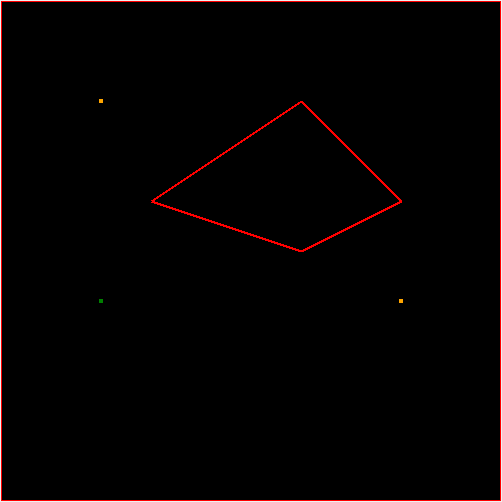
\includegraphics[scale=0.4]{scenario1}
	\caption{Scenariusz testowy 1}
	\label{fig:sc1}
\end{figure}

\begin{figure}[h!]
	\centering
	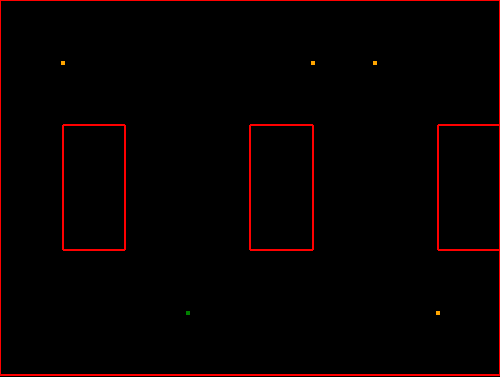
\includegraphics[scale=0.4]{scenario2}
	\caption{Scenariusz testowy 2}
	\label{fig:sc2}
\end{figure}

\begin{figure}[h!]
	\centering
	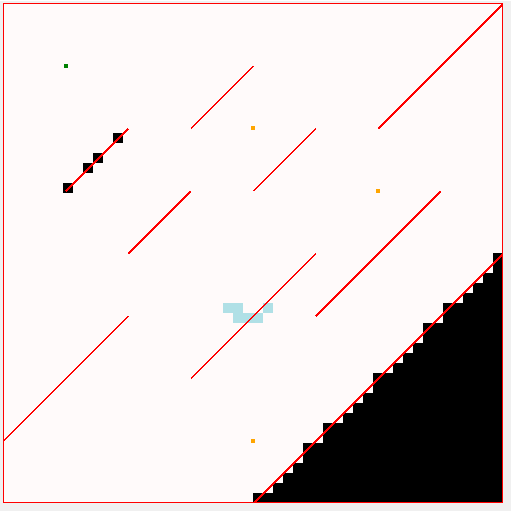
\includegraphics[scale=0.4]{scenario3}
	\caption{Scenariusz testowy 3}
	\label{fig:sc3}
\end{figure}

\begin{figure}[h!]
	\centering
	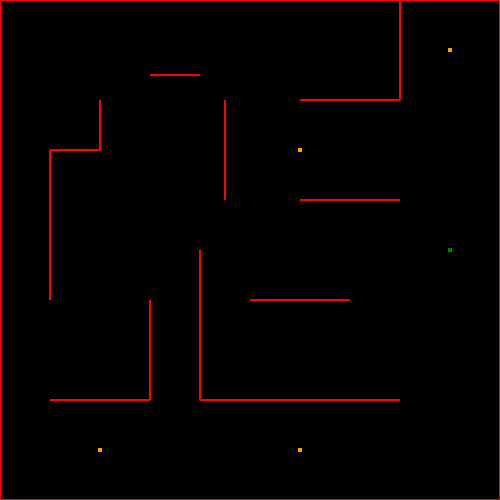
\includegraphics[scale=0.4]{scenario4}
	\caption{Scenariusz testowy 4}
	\label{fig:sc4}
\end{figure}

\begin{figure}[h!]
	\centering
	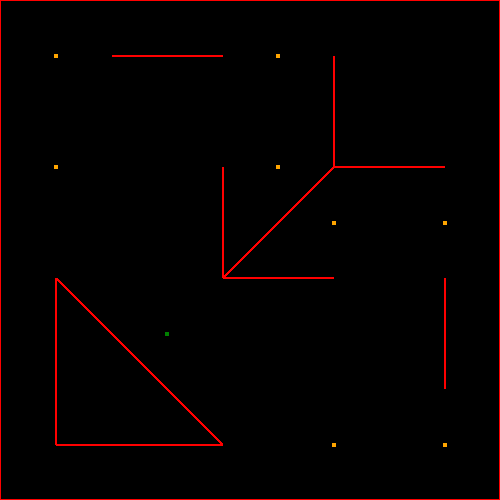
\includegraphics[scale=0.4]{scenario5}
	\caption{Scenariusz testowy 5}
	\label{fig:sc5}
\end{figure}

\subsection{Wyniki}
Algorytm dość szybko znajduje osobniki które są bliskie rozwiązaniom optymalnym. Niestety od pewnego momentu wyniki przestają być poprawiane mimo wywoływania tysięcy iteracji algorytmu. Jest to zapewne skutkiem operatora mutacji, który (pomimo zastosowanych rozwiązań) ma kłopot ze zmianą kątów o małe wartości. Mimo to ogólne tendencje ewolucji osobników pokazują, że algorytm jest na dobrej drodze do znalezienia osobników optymalnych.

Należy jednak zwrócić uwagę na fakt, że dla struktury drzewiastej, każdy scenariusz ma dokładnie jedno rozwiązanie optymalne, podczas gdy zarówno w standardowym zagadnieniu kinematyki odwrotnej jak i wersji zmodyfikowanej z podziałem na ramię i palce, takich rozwiązań w większości scenariuszy istnieje nieskończenie wiele. Wynika to z~tego, że punkty docelowe są ściśle przywiązane do liści, a~każdy węzeł jest związany z co najmniej dwoma końcami efektora, musi mieć więc jednoznaczne ustawienie i nawet niewielkie odchylenia miar kątów mają w~tym przypadku kluczowe znaczenie. Tak więc, ze względu na naturę problemu, znalezienie bezbłędnych osobników bliskich rozwiązaniu optymalnemu wydaje się dobrym osiągnięciem.


\section{Podsumowanie}
Podsumowując, rozszerzenie pojęcia osobnika z łamanej do drzewa po pierwsze diametralnie zmniejsza liczbę optymalnych rozwiązań, po drugie wprowadza szereg problemów przy projektowaniu operatorów ewolucyjnych. Z~powodu komplikacji struktury osobnika pojawia się wiele możliwych rozwiązań podczas projektowania operatorów krzyżowania i mutacji, nie są one jednak uniwersalne. Znika możliwość stworzenia jednego ogólnego algorytmu działającego przez wszystkie pokolenia i pojawia się konieczność tworzenia dedykowanych operatorów dla konkretnych sytuacji, które to operatory pozwolą na optymalny rozwój populacji w kierunku rozwiązania optymalnego.


\begin{thebibliography}{1}
	\bibitem{PFI} Patryk Filipiak, {\it Optymalizacja ewolucyjna z predykcją w dynamicznym problemie kinematyki odwrotnej}. Wrocław, Seminarium ZMN IIUWr 2011.
\end{thebibliography}

\end{document}